%%%%%%%%%%%%%%%%%%%%%%%%%%%%%%%%%%%%%%%%%%%%%%%%%%%%%%%%%%%%%%%%%%%%%%
% Template para artigos da SBC
% Adaptado para o trabalho prático de Processamento de Dados com Grafos
%%%%%%%%%%%%%%%%%%%%%%%%%%%%%%%%%%%%%%%%%%%%%%%%%%%%%%%%%%%%%%%%%%%%%%

\documentclass[12pt]{article}

\usepackage{sbc-template}
\usepackage{graphicx,url}
\usepackage[utf8]{inputenc}  
\usepackage{amsmath} % Para ambientes matemáticos
\usepackage{listings} % Para blocos de código
\usepackage{xcolor} % Para cores no código

% Configuração para blocos de código
\definecolor{codegreen}{rgb}{0,0.6,0}
\definecolor{codegray}{rgb}{0.5,0.5,0.5}
\definecolor{codepurple}{rgb}{0.58,0,0.82}
\definecolor{backcolour}{rgb}{0.95,0.95,0.92}

\lstdefinestyle{customStyle}{
    backgroundcolor=\color{backcolour},   
    commentstyle=\color{codegreen},
    keywordstyle=\color{magenta},
    numberstyle=\tiny\color{codegray},
    stringstyle=\color{codepurple},
    basicstyle=\ttfamily\footnotesize,
    breakatwhitespace=false,         
    breaklines=true,                 
    captionpos=b,                    
    keepspaces=true,                 
    numbers=left,                    
    numbersep=5pt,                  
    showspaces=false,                
    showstringspaces=false,
    showtabs=false,                  
    tabsize=2
}
\lstset{style=customStyle}
     
\sloppy

\title{Gestão de Dependências em Projetos Go com Ordenação Topológica}

% TODO: PREENCHER OS DADOS DOS AUTORES E INSTITUIÇÕES
\author{Nicholas Pereira Cristófaro\inst{1}, Nome Sobrenome do Aluno 2\inst{1}}

\address{Pontifícia Universidade Católica de Minas Gerais\\
  Belo Horizonte -- Minas Gerais -- Brasil
  \email{nicholaspcr@gmail.com, email2@dominio.com}
}

\begin{document} 

\maketitle

\begin{resumo} 
  A complexidade crescente dos sistemas de software modernos exige mecanismos robustos para a gestão de dependências. Este artigo apresenta o desenvolvimento de uma ferramenta para análise e visualização de dependências em projetos na linguagem Go. O problema da ordem de inicialização de pacotes é modelado como um grafo direcionado, onde os pacotes são os vértices e as importações representam as arestas. Utilizando o algoritmo de Kahn para ordenação topológica, a ferramenta determina a sequência de compilação segura e identifica a existência de dependências cíclicas, um erro crítico em Go. O trabalho detalha a implementação em Python, desde a análise do código-fonte até a geração de uma visualização gráfica interativa do grafo, alinhando-se ao tema de gestão de conflitos em sistemas de dependência.
\end{resumo}

\begin{abstract}
  The growing complexity of modern software systems demands robust mechanisms for dependency management. This paper presents the development of a tool for analyzing and visualizing dependencies in projects written in the Go language. The package initialization order problem is modeled as a directed graph, where packages are vertices and imports represent edges. Using Kahn's algorithm for topological sorting, the tool determines the safe compilation sequence and identifies the existence of cyclic dependencies, a critical error in Go. The work details the Python implementation, from source code parsing to the generation of an interactive graphical visualization of the graph, aligning with the theme of conflict management in dependency systems.
\end{abstract}


\section{Introdução}

O desenvolvimento de software contemporâneo é caracterizado pela modularidade e reutilização de código, resultando em sistemas compostos por um grande número de componentes interdependentes. A gestão dessa rede de dependências é um desafio central na engenharia de software. Falhas nesse gerenciamento podem levar a erros de compilação, comportamento inesperado em tempo de execução e dificuldades na manutenção e evolução dos projetos.

A linguagem de programação Go (Golang), desenvolvida pelo Google, possui um sistema de pacotes estático e um compilador que impõem regras estritas sobre as dependências. Uma dessas regras é que as dependências de um pacote devem ser inicializadas antes do próprio pacote. Isso garante a execução correta das funções `init()`, que são utilizadas para configurar o estado inicial de cada pacote. Quando um projeto contém uma dependência cíclica (por exemplo, pacote A importa B e pacote B importa A), o compilador Go gera um erro, pois não é possível determinar uma ordem de inicialização válida.

A ordem de inicialização de pacotes em Go pode ser modelada de forma natural como um grafo de dependências direcionado acíclico (DAG). Neste modelo, cada pacote é um vértice e uma diretiva `import` de um pacote A para um pacote B cria uma aresta direcionada de B para A, significando que A depende de B. A solução para determinar a sequência correta de inicialização é, portanto, encontrar uma ordenação topológica desse grafo.

Este trabalho se enquadra na proposta de "Gestão de Conflitos em Sistemas de Dependência", focando na modelagem, detecção de ciclos e execução segura baseada em ordenação topológica. Para isso, foi desenvolvida uma ferramenta em Python que:
\begin{itemize}
    \item Analisa recursivamente os arquivos de um projeto Go para extrair as relações de importação.
    \item Constrói um grafo de dependências direcionado a partir dessas relações.
    \item Aplica o algoritmo de Kahn para realizar a ordenação topológica dos pacotes.
    \item Gera uma visualização gráfica do grafo de dependências, destacando a ordem de inicialização em camadas.
\end{itemize}

O restante deste artigo está organizado da seguinte forma: a Seção 2 apresenta a fundamentação teórica sobre grafos, ordenação topológica e o sistema de pacotes do Go. A Seção 3 detalha a modelagem do problema e a arquitetura da ferramenta desenvolvida. A Seção 4 apresenta os experimentos realizados e discute os resultados obtidos. Finalmente, a Seção 5 conclui o trabalho e aponta direções para desenvolvimentos futuros.

\begin{figure}[ht]
\centering
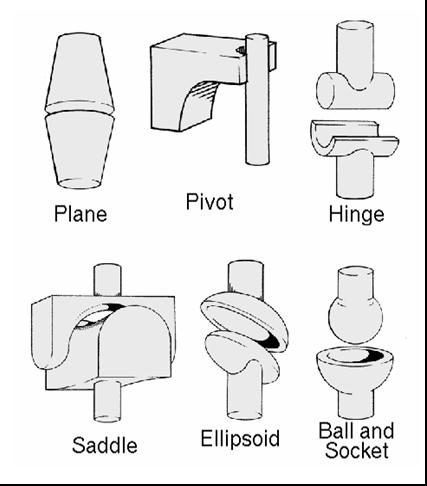
\includegraphics[width=.3\textwidth]{fig2.jpg}
\caption{Esta figura é um exemplo de uma legenda de figura que ocupa mais de uma
linha e é justificada considerando as margens mencionadas na Seção~\ref{sec:figs}.}
\label{fig:exampleFig2}
\end{figure}

Em tabelas, tente evitar o uso de fundos coloridos ou sombreados, e evite
linhas de enquadramento grossas, duplas ou desnecessárias. Ao relatar dados empíricos,
não use mais dígitos decimais do que o justificado por sua precisão e
reprodutibilidade. A legenda da tabela deve ser colocada antes da tabela (ver Tabela 1)
e a fonte usada também deve ser Helvetica, 10 pontos, negrito, com 6 pontos de
espaço antes e depois de cada legenda.

\begin{table}[ht]
\centering
\caption{Variáveis a serem consideradas na avaliação de técnicas de
interação}
\label{tab:exTable1}
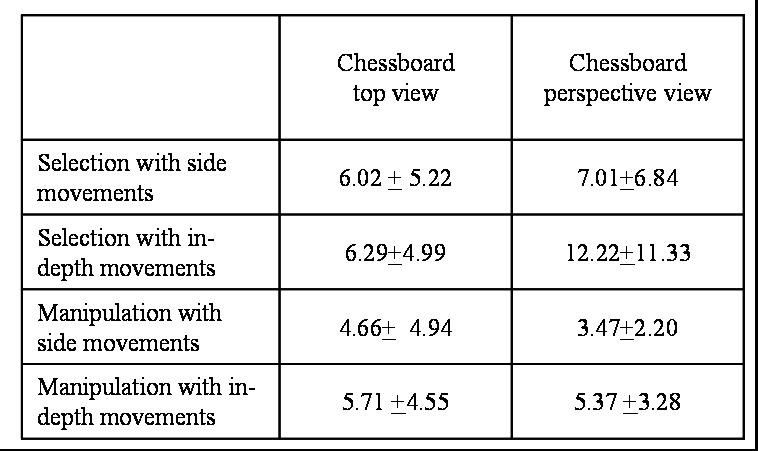
\includegraphics[width=.7\textwidth]{table.jpg}
\end{table}

\section{Imagens}

Todas as imagens e ilustrações devem ser em preto e branco, ou tons de cinza,
exceto para os artigos que estarão disponíveis eletronicamente (em CD-ROMs,
internet, etc.). A resolução da imagem no papel deve ser de cerca de 600 dpi para
imagens em preto e branco, e 150-300 dpi para imagens em tons de cinza. Não inclua
imagens com resolução excessiva, pois elas podem levar horas para imprimir, sem qualquer
diferença visível no resultado.

\section{Referências}

As referências bibliográficas devem ser inequívocas e uniformes. Recomendamos fornecer
as referências dos nomes dos autores entre colchetes, por exemplo, \cite{knuth:84},
\cite{boulic:91}, e \cite{smith:99}. As referências devem ser listadas usando fonte de tamanho 12, com 6 pontos de espaço
antes de cada referência. A primeira linha de cada referência não deve ser
recuada, enquanto as subsequentes devem ser recuadas em 0,5 cm.

\bibliographystyle{sbc}
\bibliography{sbc-template.bib}

\end{document}
